% ============================================================
%  NOT gate - breadboard wiring diagram (PUSH-PULL output).
%  Drawn the way it actually sits on a solderless breadboard:
%    - the hole grid + the two power rails (+5 V red, GND blue),
%    - three 2N3904 transistors plugged in (legs E B C, spaced out),
%    - resistors and LEDs as real components,
%    - colour-coded jumper wires (see the legend).
%  Each column of 5 holes in a bank is one electrical node.
%  Compile:  pdflatex wiring.tex
% ============================================================
\documentclass[border=16pt]{standalone}
\usepackage{circuitikz}
\usepackage{tikz}
\usetikzlibrary{calc, positioning}

\definecolor{vcc}{RGB}{205,45,45}      % +5 V wires (red)
\definecolor{gnd}{RGB}{35,35,40}       % GND wires (near-black)
\definecolor{anet}{RGB}{20,140,60}     % input A (green)
\definecolor{abar}{RGB}{235,140,0}     % A-bar (orange)
\definecolor{onet}{RGB}{120,45,175}    % output (violet)
\definecolor{board}{RGB}{246,241,229}  % breadboard body

% one TO-92 transistor, legs spaced TWO holes apart for clearance.
% #1 = column of the E leg, #2 = reference tag.
% legs go into row A holes of columns #1, #1+2, #1+4.
\newcommand{\trans}[2]{%
  \pgfmathsetmacro\xe{0.7*#1}%
  \pgfmathsetmacro\xb{0.7*(#1+2)}%
  \pgfmathsetmacro\xc{0.7*(#1+4)}%
  % body: flat bottom, rounded top
  \draw[fill=black!10]
        (\xe-0.4,9.55) -- (\xe-0.4,9.95)
        arc (180:0:{(\xc-\xe+0.8)/2} and 0.45) -- (\xc+0.4,9.55) -- cycle;
  \node[font=\footnotesize\bfseries] at (\xb,9.85) {2N3904};
  \node[font=\scriptsize,anchor=east] at (\xe-0.5,9.9) {#2};
  % legs (long, for margin)
  \draw (\xe,9.55)--(\xe,9.0);
  \draw (\xb,9.55)--(\xb,9.0);
  \draw (\xc,9.55)--(\xc,9.0);
  % E B C pin labels, centred under each (well-separated) leg
  \node[red,font=\scriptsize\bfseries,anchor=north] at (\xe,8.92) {E};
  \node[red,font=\scriptsize\bfseries,anchor=north] at (\xb,8.92) {B};
  \node[red,font=\scriptsize\bfseries,anchor=north] at (\xc,8.92) {C};
}

\begin{document}
% ONE uniform line weight for every wire, lead and rail
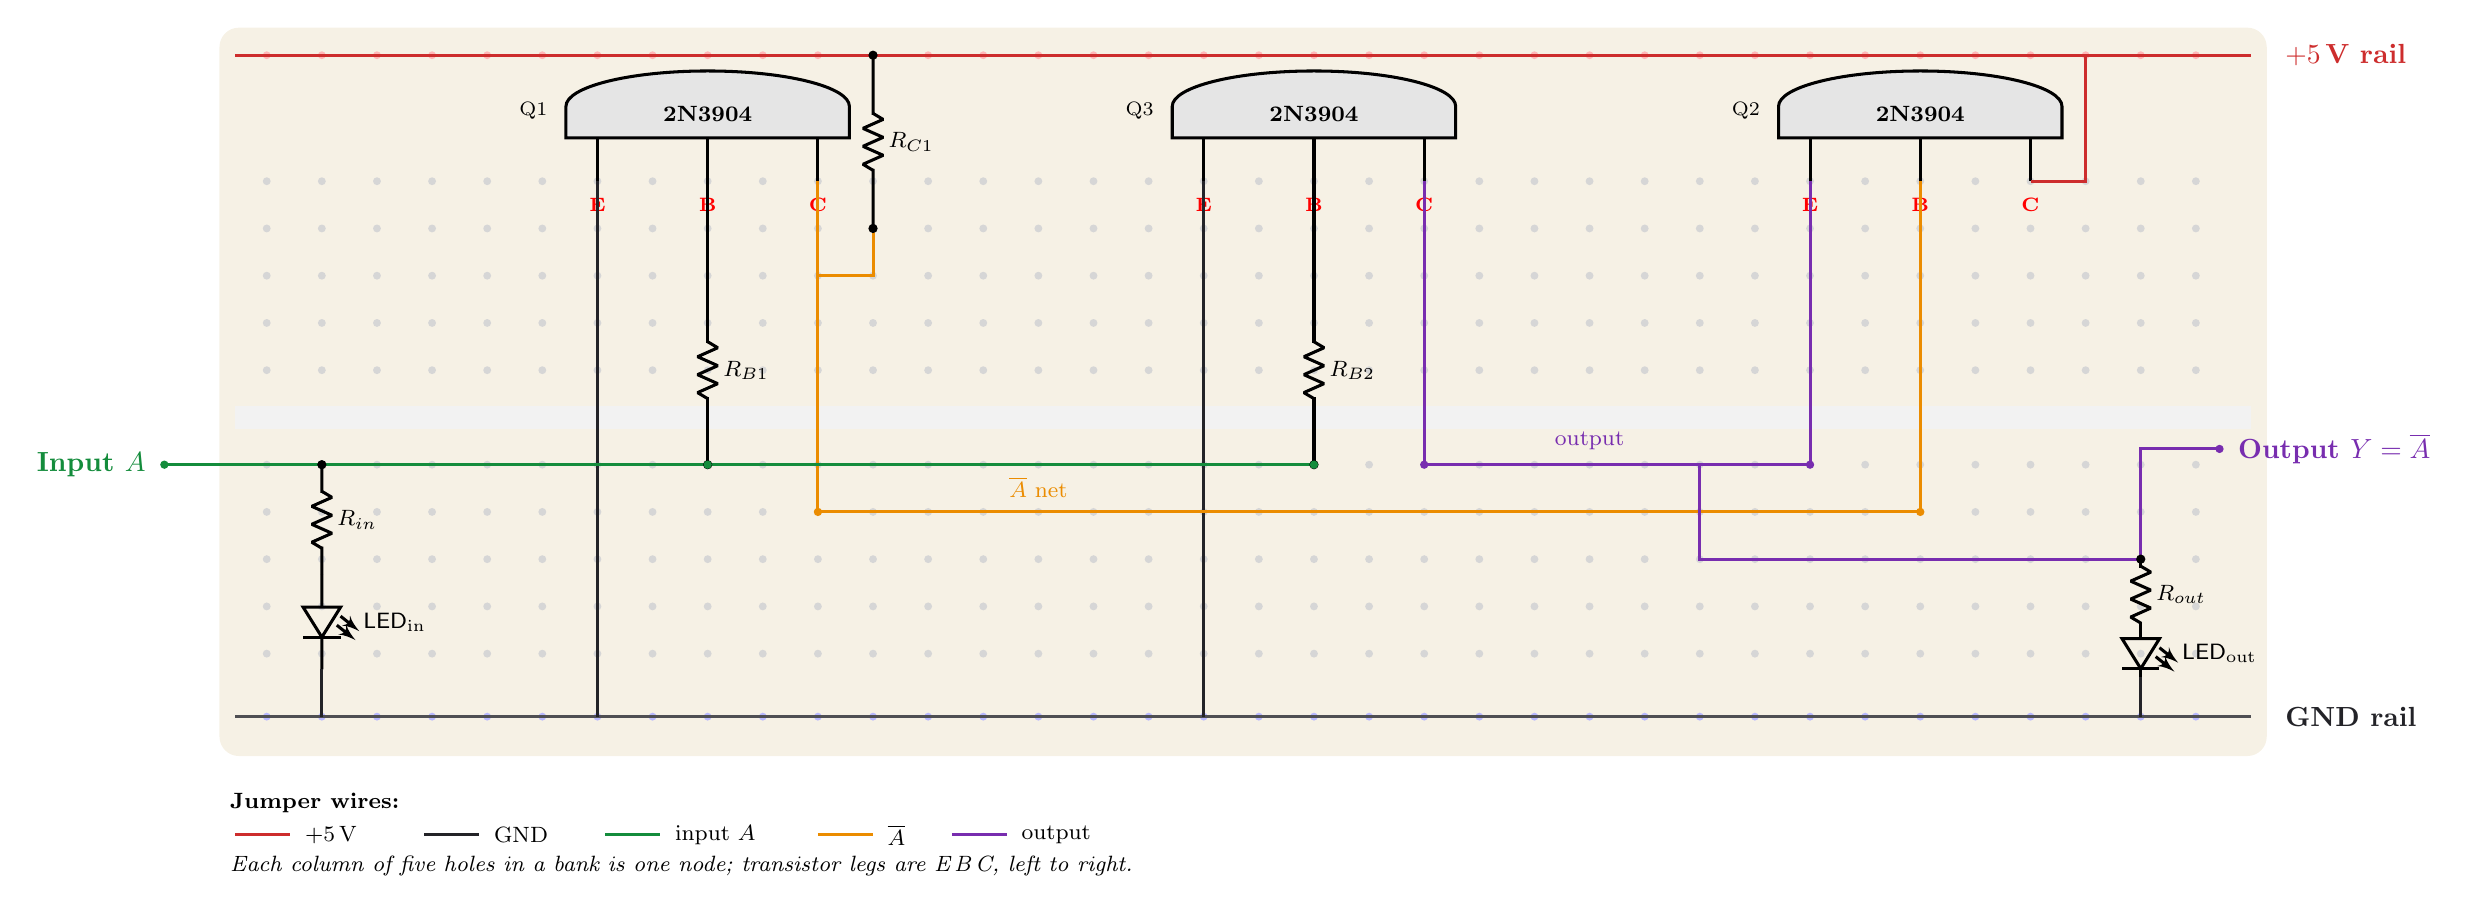
\begin{tikzpicture}[line width=1.1pt, font=\sffamily]
  \ctikzset{bipoles/thickness=1, bipoles/length=0.95cm, resistors/scale=0.9}

  % ---------- board body ----------
  \fill[board,rounded corners=7pt] (0.1,1.7) rectangle (26.1,10.95);

  % ---------- hole grid (two banks of 5 rows) ----------
  \foreach \c in {1,...,36}{
    \foreach \y in {9.0,8.4,7.8,7.2,6.6, 5.4,4.8,4.2,3.6,3.0}{
      \fill[black!16] ({0.7*\c},\y) circle (0.5mm);
    }
  }
  % centre gap (ravine)
  \fill[black!5] (0.3,5.85) rectangle (25.9,6.15);

  % ---------- power rails ----------
  \foreach \c in {1,...,36}{
    \fill[red!28]  ({0.7*\c},10.6) circle (0.5mm);
    \fill[blue!28] ({0.7*\c},2.2)  circle (0.5mm);
  }
  \draw[vcc]    (0.3,10.6) -- (25.9,10.6);
  \draw[gnd!80] (0.3,2.2)  -- (25.9,2.2);
  \node[vcc,font=\bfseries,anchor=west]  at (26.2,10.6) {$+5\,$V rail};
  \node[gnd,font=\bfseries,anchor=west]  at (26.2,2.2)  {GND rail};

  % ---------- transistors (E legs at cols 7, 18, 29 -> clear space on the left) ----------
  \trans{7}{Q1}
  \trans{18}{Q3}
  \trans{29}{Q2}

  % =========================================================
  %  GND jumpers (black):  Q1 emitter (col7) and Q3 emitter (col18)
  % =========================================================
  \draw[gnd] ({0.7*7},9.0)  -- ({0.7*7},2.2);
  \draw[gnd] ({0.7*18},9.0) -- ({0.7*18},2.2);

  % =========================================================
  %  +5 V jumper (red):  Q2 collector (col33) out past the body, up to the rail
  % =========================================================
  \draw[vcc] ({0.7*33},9.0) -- ({0.7*34},9.0) -- ({0.7*34},10.6);

  % =========================================================
  %  A-bar net (orange):  Q1 collector (col11) -> R_C1 -> +5 V, bus to Q2 base (col31)
  % =========================================================
  \draw[abar] ({0.7*11},9.0) -- ({0.7*11},4.8);
  \draw[abar] ({0.7*11},7.8) -- ({0.7*12},7.8) -- ({0.7*12},8.4);
  \draw ({0.7*12},8.4) to[R, l_=\footnotesize $R_{C1}$, *-*] ({0.7*12},10.6);
  \draw[abar] ({0.7*11},4.8) -- ({0.7*31},4.8);
  \draw[abar] ({0.7*31},9.0) -- ({0.7*31},4.8);
  \fill[abar] ({0.7*11},4.8) circle (1.5pt);
  \fill[abar] ({0.7*31},4.8) circle (1.5pt);
  \node[abar,font=\footnotesize,anchor=south] at ({0.7*15},4.85) {$\overline{A}$ net};

  % =========================================================
  %  INPUT A net (green):  input -> bus (col2..col20); R_B1 -> Q1 base, R_B2 -> Q3 base; LED
  % =========================================================
  \draw[anet] (-0.6,5.4) -- ({0.7*20},5.4);
  \node[anet,anchor=east,font=\bfseries] at (-0.7,5.4) {Input $A$};
  \fill[anet] (-0.6,5.4) circle (1.5pt);
  % R_B1: A bus -> Q1 base (col9)
  \draw ({0.7*9},9.0) -- ({0.7*9},7.8);
  \draw ({0.7*9},7.8) to[R, l=\footnotesize $R_{B1}$, -*] ({0.7*9},5.4);
  \fill[anet] ({0.7*9},5.4) circle (1.5pt);
  % R_B2: A bus -> Q3 base (col20)
  \draw ({0.7*20},9.0) -- ({0.7*20},7.8);
  \draw ({0.7*20},7.8) to[R, l=\footnotesize $R_{B2}$, -*] ({0.7*20},5.4);
  \fill[anet] ({0.7*20},5.4) circle (1.5pt);
  % input LED branch on col2 (clear space on both sides):  A -> R_in -> LED -> GND
  \fill[anet] ({0.7*2},5.4) circle (1.5pt);
  \draw ({0.7*2},5.4) to[R, l=\footnotesize $R_{in}$, *-] ({0.7*2},4.0);
  \draw ({0.7*2},4.0) to[leD, l=\footnotesize LED$_{\mathrm{in}}$] ({0.7*2},2.8);
  \draw[gnd] ({0.7*2},2.8) -- ({0.7*2},2.2);

  % =========================================================
  %  OUTPUT net (violet):  Q3 collector (col22) + Q2 emitter (col29); terminal + LED
  % =========================================================
  \draw[onet] ({0.7*22},9.0) -- ({0.7*22},5.4);
  \draw[onet] ({0.7*29},9.0) -- ({0.7*29},5.4);
  \draw[onet] ({0.7*22},5.4) -- ({0.7*29},5.4);
  \fill[onet] ({0.7*22},5.4) circle (1.5pt);
  \fill[onet] ({0.7*29},5.4) circle (1.5pt);
  \node[onet,font=\footnotesize,anchor=south] at ({0.7*25},5.45) {output};
  % carry the output out to the right past Q2, in a clear low channel
  \draw[onet] ({0.7*27},5.4) -- ({0.7*27},4.2) -- ({0.7*35},4.2);
  \draw[onet] ({0.7*35},4.2) -- ({0.7*35},5.6) -- (25.5,5.6);
  \node[onet,anchor=west,font=\bfseries] at (25.6,5.6) {Output $Y=\overline{A}$};
  \fill[onet] (25.5,5.6) circle (1.5pt);
  % output LED branch on col35:  OUT -> R_out -> LED -> GND
  \draw ({0.7*35},4.2) to[R, l=\footnotesize $R_{out}$, *-] ({0.7*35},3.3);
  \draw ({0.7*35},3.3) to[leD, l=\footnotesize LED$_{\mathrm{out}}$] ({0.7*35},2.7);
  \draw[gnd] ({0.7*35},2.7) -- ({0.7*35},2.2);

  % =========================================================
  %  legend
  % =========================================================
  \begin{scope}[shift={(0.3,0.55)}]
    \node[anchor=west,font=\footnotesize\bfseries] at (-0.2,0.55) {Jumper wires:};
    \draw[vcc]  (0.0,0.15)--(0.7,0.15); \node[anchor=west,font=\footnotesize] at (0.75,0.15){+5\,V};
    \draw[gnd]  (2.4,0.15)--(3.1,0.15); \node[anchor=west,font=\footnotesize] at (3.15,0.15){GND};
    \draw[anet] (4.7,0.15)--(5.4,0.15); \node[anchor=west,font=\footnotesize] at (5.45,0.15){input $A$};
    \draw[abar] (7.4,0.15)--(8.1,0.15); \node[anchor=west,font=\footnotesize] at (8.15,0.15){$\overline{A}$};
    \draw[onet] (9.1,0.15)--(9.8,0.15); \node[anchor=west,font=\footnotesize] at (9.85,0.15){output};
    \node[anchor=west,font=\footnotesize\itshape] at (-0.2,-0.25)
        {Each column of five holes in a bank is one node; transistor legs are E\,B\,C, left to right.};
  \end{scope}

\end{tikzpicture}
\end{document}
